\documentclass[11pt,a4paper,sans]{moderncv}

\moderncvstyle{casual}
\moderncvcolor{blue}
%\nopagenumbers{}

\usepackage[utf8]{inputenc}
\usepackage[T1]{fontenc}
\usepackage[french]{babel}

% adjust the page margins
\usepackage[scale=0.75]{geometry}
%\setlength{\hintscolumnwidth}{3cm}                % if you want to change the width of the column with the dates
%\setlength{\makecvtitlenamewidth}{10cm}           % for the 'classic' style, if you want to force the width allocated to your name and avoid line breaks. be careful though, the length is normally calculated to avoid any overlap with your personal info; use this at your own typographical risks...
\graphicspath{{figures/}}
% personal data
\name{Vincent}{Lafouasse}
\title{B.Sc. in Chemistry}
\address{28 square du clos de Villaine}{91300 Massy}{\textsc{France}}
\phone[mobile]{+33 6 21 59 25 74}
\phone[fixed]{+33 9 50 40 28 82}
\email{vincentlafouasse@live.fr}
%\homepage{www.johndoe.com}
%\social[linkedin]{john.doe}
%\social[twitter]{jdoe}
%\social[github]{jdoe}
%\extrainfo{additional information}
%\photo[64pt][0.4pt]{picture}                       % optional, remove / comment the line if not wanted; '64pt' is the height the picture must be resized to, 0.4pt is the thickness of the frame around it (put it to 0pt for no frame) and 'picture' is the name of the picture file
%\quote{Some quote}                                 % optional, remove / comment the line if not wanted

% bibliography adjustements (only useful if you make citations in your resume, or print a list of publications using BibTeX)
%   to show numerical labels in the bibliography (default is to show no labels)
\makeatletter\renewcommand*{\bibliographyitemlabel}{\@biblabel{\arabic{enumiv}}}\makeatother
%   to redefine the bibliography heading string ("Publications")
%\renewcommand{\refname}{Articles}

% bibliography with mutiple entries
%\usepackage{multibib}
%\newcites{book,misc}{{Books},{Others}}
%----------------------------------------------------------------------------------
%            content
%----------------------------------------------------------------------------------
\begin{document}

\makecvtitle


\section{Research Interest}
\cvitem{}{I am mainly interested in the field of Molecular Chemistry, especially Organic Synthesis, Total Synthesis and Supramolecular Chemistry}


\section{Education}
\cventry{2018--now}{Master (M.Sc.)}{Université Paris-Sud}{Orsay (91)}{}{Organic Chemistry platform\vspace {1mm}%\newline{}%
%Classes :%
%\vspace{2mm}
%\begin{itemize}%
%\item D4CI430: Sélectivités en synthèse organique et chimie organométallique
%\item D4CI431: Les réactions fondamentales appliquées aux architectures carbonées
%\item D4CI434: Stratégies et outils en synthèse organique avancée
%\item D4CI438: Synthèses de molécules organiques issues du vivant \vspace{5mm}
%\item D4CI401: Caractérisation structurale par RMN et diffraction X (Socle Commun)
%\item D4CI402: Sol-gel, surfaces et fonctionnalisations organiques (Socle Commun)
%\item D4CI405: Techniques d’analyse (chromatographies, spectrométrie de masse, spectroscopies optiques) (Tronc Commun UPSUD)
%\end{itemize}
}
%
\cventry{2017--2018}{Bachelor (B.Sc.)}{Sorbonne Université}{Paris (75)}{\textit{}}{Fundamentals of Chemistry and Physics}
%
\cventry{2015--2017}{Bachelor (B.Sc.)}{Ecole Normale Supérieure de Lyon}{Lyon (69)}{\textit{}}{élève normalien : A unique, non-specialized training program in Physics and Chemistry}

\cventry{2013--2015}{Classe Préparatoires (CPGE)}{Lycée Henri IV}{Paris (75)}{\textit{}}{PCSI/PC$^*$ : Two years of intensive theoretical courses in Mathematics, Physics and Chemistry in order to prepare for école Normale Supérieure national selective exam}

\cventry{2013}{Baccalauréat (A-levels)}{Lycée de l'Île-de-France}{Villebon-sur-Yvette (91)}{}{Science major, Highest Honours}


\section{Experience}


\subsection{Research}

\cventry{2020}{4 month internship}{ICMMO (UMR 8182)}{Orsay (91)}{Electrocatalysis and CO$_2$ valorization}{Under the direction of Mohamed Mellah and Emmanuelle Schulz\newline{}%
Préparation de dérivés de type acide 2-phénylpropanoïque énantioenrichis, en partant d'halogénures benzéniques secondaires par activation du CO2 en présence de quantités catalytiques de Sm(II) électrogénéré
}


\cventry{2018}{Lab week}{Sorbonne Université}{Paris (75)}{Supramolecular Chemistry}{Under the direction of Matthieu Sollogoub (IPCM, GOBS) as part of the UE 3C015 TEOREM\newline{}%
Detailed achievements:%
\begin{itemize}%
\item Study of $\beta$-CD based inclusion compounds
\item Synthesis and RMN caracterisation of a $\alpha$-CD based [3]-rotaxane
\item Synthesis and RMN caracterisation of a self-assembled iron cage
\end{itemize}
}

\cventry{2014-2015}{TIPE}{Lycée Henri IV}{Paris (75)}{Supramolecular Chemistry}{Under the direction of Julien Lalande \newline{}%
Detailed achievements:%
\begin{itemize}%
\item Synthesis of dibenzo-18-crown-6 using Pedersen's original protocol
\item Qualitative and quantitative study of crown ether complexes with different cations
\end{itemize}
}


\subsection{Teaching}
\cventry{2018--now}{Chemistry Professor}{Optimal Sup Spé}{Paris (75)}{}{Teaching groups of CPGE students from all scientific tracks (PC, MP, PSI, BCPST)\newline{}%
Detailed achievements:%
\begin{itemize}%
\item +12h of formation and +200 h of class
\item \LaTeX $~$edition
\item Preparation of students for the national entrance exams to XENS
\end{itemize}
}


\section{Languages}
\cvitemwithcomment{French}{Fluent}{Native speaker}
\cvitemwithcomment{English}{Fluent}{C2 BULATS 05/18}


\section{Skills}
\cvitem{Molecular Chemistry}{Organic Synthesis, Total Synthesis, Supramolecular Chemistry }
\cvitem{General Chem}{Quantum Chemistry, Spectroscopy, Cristallography }
\cvitem{Physics}{Quantum Mechanics, Thermodynamics }
\cvitem{Programming}{Python
\includegraphics[height=1.4\fontcharht\font`\B]{python_logo.png}, {\LaTeX}, Julia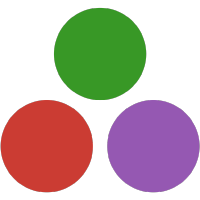
\includegraphics[height=1.4\fontcharht\font`\B]{julia_logo.png}, C}

\section{Interests}
\cvitem{Music}{Jazz guitar, Trumpet}
\cvitem{}{Music theory and Jazz harmony}
\cvitem{}{Dance}



\clearpage

\end{document}
